\section{Results}\label{sec:results}

The proposed model is tested on three aspects with the experiments mentioned above. The global noise and label shuffling experiments test whether the model can predict its variance accordingly. The experiment on localized noise checks whether the location of noise affects the predicted variance. Lastly, the traceable noise experiment checks whether the source of uncertainty can be located using Shapley values.

\subsection{Base variance predictions}

Figure \ref{fig:histogram} shows the distribution of the predicted variances on correct and incorrect predictions. From this histogram, one can observe that the model's classification is almost always correct when it is paired with a low variance prediction. The higher the model's predicted variance becomes, the more often the classification is incorrect. Although the two histograms overlap, there is a clear skew towards higher variances for the incorrect predictions. On the highest variance predictions ranging from $0.24$ to $0.25$, the distribution between correct and incorrect classifications is nearly equal, indicating that the model is randomly guessing the classification.

\begin{figure}[!tbp]
    \centering
        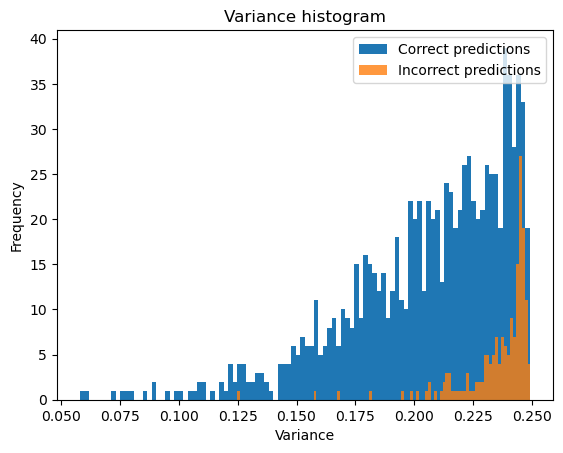
\includegraphics[width=7.7cm]{img/histogram.png}
    \caption{Histogram with the frequencies of variance predictions for correct and incorrect predictions. A higher predicted variance indicates a higher probability of an incorrect prediction.}
    \label{fig:histogram}
\end{figure}


\subsection{General noise}

Figure \ref{fig:label_shuffle} shows the effect of shuffling the labels of training and testing data on the model's predicted variance. Here, it is clear that there is an increase in predicted variance as more labels in the training and testing set are shuffled. However, this difference is not very large, with only an increase of approximately $0.027$, with a relatively high difference between runs. The overall behavior of the variance's head output is as expected: as more labels are shuffled, and thus the worse the data becomes and the stronger the uncertainty gets, increasing the predicted variance.

\begin{figure}[!tbp]
    \centering
        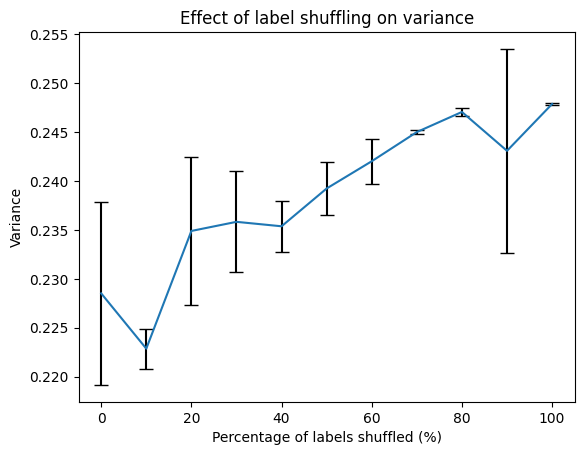
\includegraphics[width=7.7cm]{img/label_shuffle.png}
    \caption{The effect of label shuffling on the output of the variance head. An increase in the percentage of labels shuffled results in an increase of the predicted variance.}
    \label{fig:label_shuffle}
\end{figure}


Figure \ref{fig:general} shows two measurements of the model. The two plots on the left show the predicted variance of the model, whereas the two plots on the right show the model's accuracy. The top plots show the behavior when Gaussian noise is added to the entire signal length, whereas the bottom plots show the behavior when channels are entirely zeroed. The x-axis here represents the \verb|severity|, which indicates the strength of the noise. Higher values indicate that the added noise is of higher magnitude (in the case of Gaussian noise), occurring in more channels per episode and affecting more episodes in general.

As can be seen from these plots, there is an apparent increase in the predicted variance as the severity of the noise increases. This increase is present for the Gaussian noise and zeroing methods. Furthermore, there is an apparent decrease in accuracy as the severity of the noise increases. This behavior is also present for both types of noise. However, like the previous experiment, it is paired with a high difference between runs.

\begin{figure}[!tbp]
    \centering
        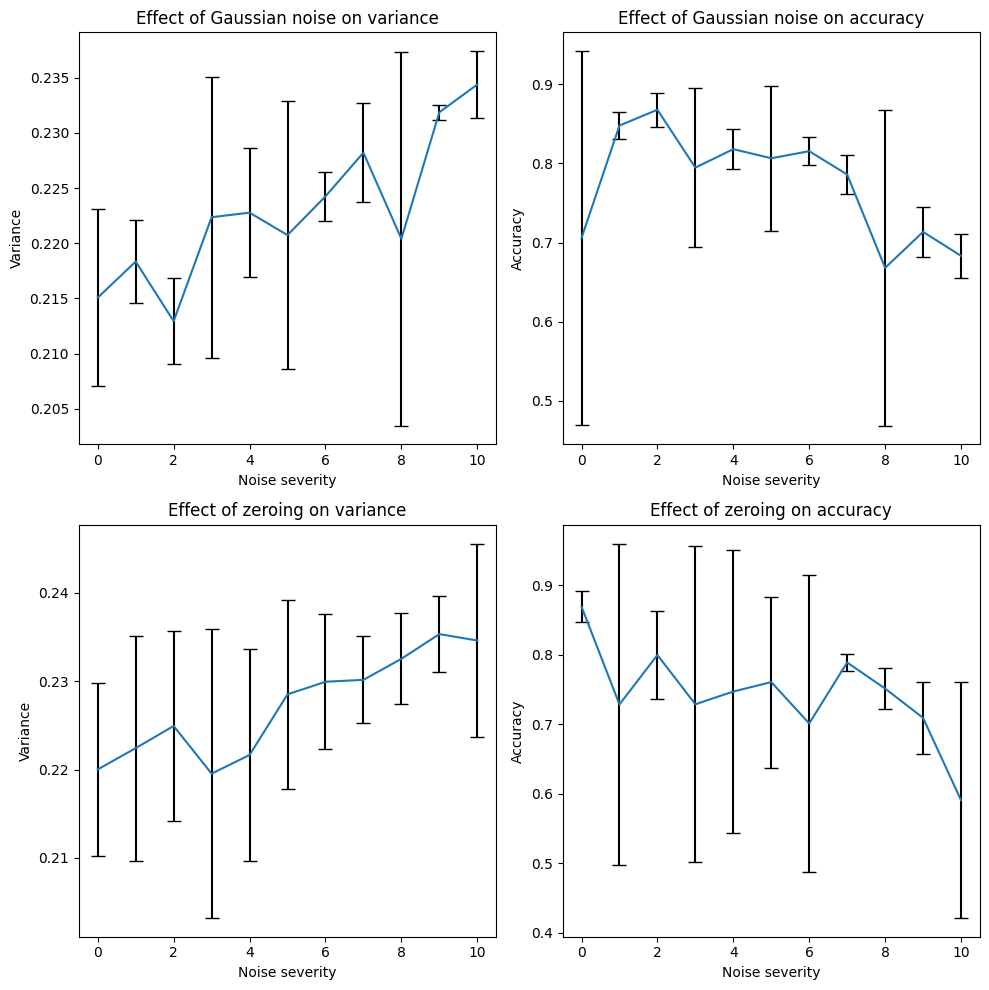
\includegraphics[width=7.7cm]{img/general.png}
    \caption{The effect of different intensities of artificial noise added to the entire signal length on the model's accuracy and variance. A higher intensity of noise results in higher predicted variance and lower accuracy.}
    \label{fig:general}
\end{figure}

\subsection{Localized noise}

Figure \ref{fig:local} shows the effect of localized noise on the variance and accuracy of the model. Here, the plots on the left show the predicted variance of the model, whereas the plots on the right show the model's accuracy. The top plots show the behavior when Gaussian noise is added to the data, whereas the bottom plots show the behavior when channels are zeroed. The left bar shows the effect of noise added on the 0-250ms region, whereas the right bar shows the effect of noise added on the 250-500ms region.

As can be observed from these plots, the general trend for both models is that the variance is higher when noise is added to the 250-500 ms region than the 0-250 ms region. For Gaussian noise, the accuracy is slightly lower when the noise is added to the 250-500 ms region than the 0-250 ms region. For the zeroed signal, the accuracy is decreased by approximately $20\%$. This shows that zeroing has a more substantial effect on the accuracy and variance. This behavior is according to expectation. When a signal has Gaussian noise added to it, the original signal still contributes to this resulting noisy signal. When a signal is zeroed, the original signal has no contribution to this resulting signal. Moreover, when averaging many signals corrupted with Gaussian noise, the noise will balance each other out. With zeroing, this does not happen. The observation that noise on the 250-500 ms region influences the accuracy and variance compared to the 0-250 ms region is as expected, as previous research showed that the most prominent part of the \verb|ErrP| signal occurs within this window \citep{lopes2021online, omedes2015analysis}. 


However, the difference in variance between the two regions is minimal, with only a $0.01$ increase for the zeroed signal and even less for the signal with Gaussian noise. And similar to the previous experiments, it is paired with a high difference between runs.

\begin{figure}[!tbp]
    \centering
        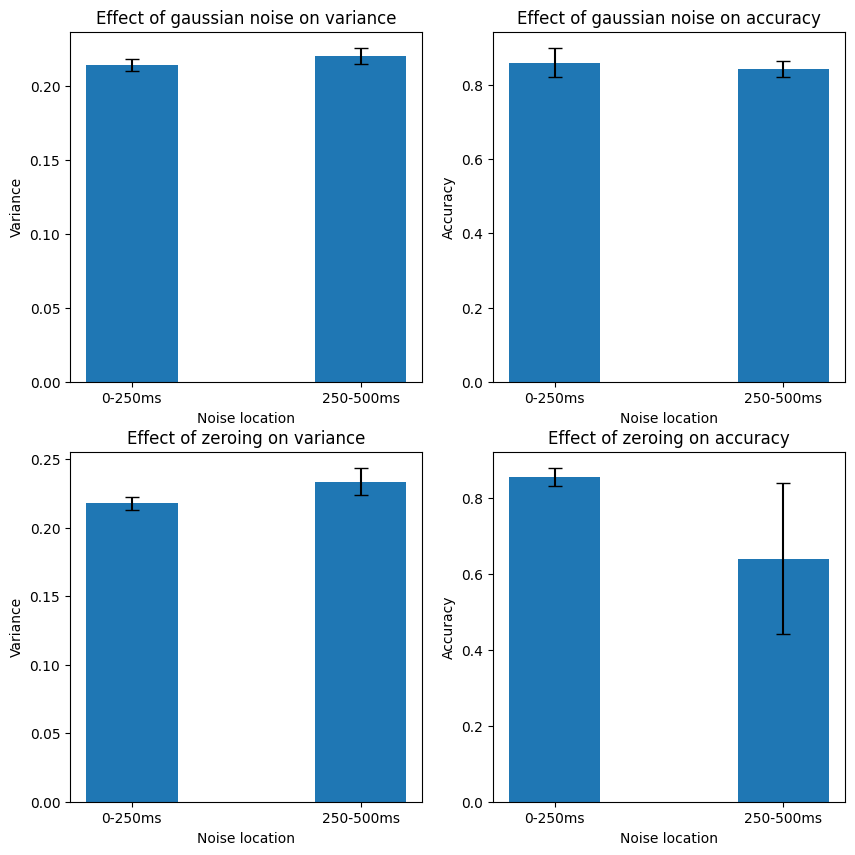
\includegraphics[width=7.7cm]{img/local.png}
    \caption{The effect of strong noise added to two different regions of the signal on the accuracy and variance of the model. Noise added to the 0-250ms region results in a higher predicted variance and lower accuracy than noise in the 250-500ms region.}
    \label{fig:local}
\end{figure}

\subsection{Traceable noise}

Figure \ref{fig:shap} shows the Shapley values of the predictions of the ErrP variance head on ErrP signals. They have been averaged over 10 trials and across all channels. Furthermore, a rolling average is used to reduce local oscillations. The left plot shows the Shapley values of the data to which Gaussian noise has been added. The right plot shows the Shapley values of the data where sections have been zeroed. Values above zero indicate a positive contribution to the variance prediction. Whereas values below zero indicate a negative contribution.

Comparing the Shapley values of the models yields various interesting observations. Firstly, when comparing the values from the model trained on the noisy data, shown in orange and green, to the one trained on the original data, shown in blue, we observe a noticeable difference between the Shapley values. From the models trained on data modified with Gaussian noise, it is clear that the Shapley values have an oscillating behavior, which the original model does not show. This oscillating behavior originates from the large differences between adjacent data points introduced by the Gaussian noise. When taking the Shapley values of many episodes, this behavior will reduce since the Gaussian noise is averaged out. However, the computational cost of approximating these Shapley values is very high. Thus the plot only shows a mean of 10 test episodes. Interestingly, the two Gaussian models have an overlapping peak of contribution, regardless of the position the noise has been added to, which is not present in the original signal. This is also visible in the zeroed models but is less significant. This behavior is unexpected, and there is most likely some underlying relation causing this, which we are not aware of.

As mentioned before, we expect an increase in the contribution to the predicted variance for the noisy models on the sections the noise has been added to. For both plots, this increase is not clearly visible. As for the Shapley values from the models trained on data modified with Gaussian noise, there is a slight increase in contribution in the 0-250ms region on inputs with noise in this area. However, in the 250-500ms region, the contributions are nearly equal. The same behavior is seen for the zeroed models, with the noise in the latter region even showing a lower contribution in that region. 


\begin{figure}[!tbp]
    \centering
        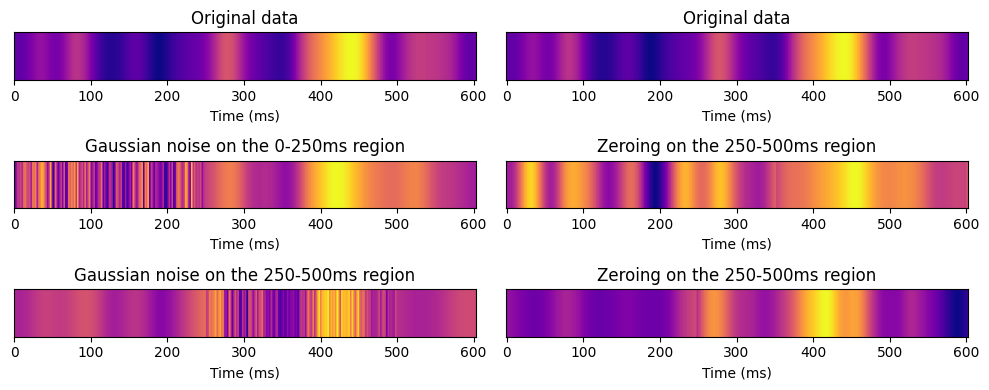
\includegraphics[width=7.7cm]{img/shap.png}
    \caption{The Shapley values of the various models. The left plot shows the Shapley values of Gaussian noise data, and the right plot shows the values of data with zeroed sections. Values above 0 (the black line) indicate a positive contribution, and all values below 0 indicate a negative contribution.}
    \label{fig:shap}
\end{figure}
